\documentclass[12pt]{article}
\usepackage[danish]{babel}
\usepackage{amsfonts, amssymb, mathtools, amsthm, amsmath}
\usepackage{graphicx, pgfplots}
\usepackage{url}
\usepackage[dvipsnames]{xcolor}
\usepackage{sagetex}

%loaded last
\usepackage[hidelinks]{hyperref}

\usepackage{siunitx}
  \sisetup{exponent-product = \cdot,
    output-decimal-marker = {,}}

%Giles Castelles incfig
\usepackage{import}
\usepackage{xifthen}
\usepackage{pdfpages}
\usepackage{transparent}

\newcommand{\incfig}[2][1]{%
  \def\svgwidth{#1\columnwidth}
  \import{../figures/}{#2.pdf_tex}
}

\setlength{\parindent}{0in}
\setlength{\oddsidemargin}{0in}
\setlength{\textwidth}{6.5in}
\setlength{\textheight}{8.8in}
\setlength{\topmargin}{0in}
\setlength{\headheight}{18pt}

\usepackage{fancyhdr}
\pagestyle{fancy}

\fancyhead{}
\fancyfoot{}
\fancyfoot[R]{\thepage}
\fancyhead[C]{\leftmark}

\pgfplotsset{compat=newest}

\pgfplotsset{every axis/.append style={
  axis x line=middle,    % put the x axis in the middle
  axis y line=middle,    % put the y axis in the middle
  axis line style={<->,color=black}, % arrows on the axis
}}

\usepackage{thmtools}
\usepackage{tcolorbox}
  \tcbuselibrary{skins, breakable}
  \tcbset{
    space to upper=1em,
    space to lower=1em,
  }

\theoremstyle{definition}

\newtcolorbox[auto counter]{definition}[1][]{%
  breakable,
  colframe=ForestGreen,  %frame color
  colback=ForestGreen!5, %background color
  colbacktitle=ForestGreen!25, %background color for title
  coltitle=ForestGreen!70!black,  %title color
  fonttitle=\bfseries\sffamily, %title font
  left=1em,              %space on left side in box,
  enhanced,              %more options
  frame hidden,          %hide frame
  borderline west={2pt}{0pt}{ForestGreen},  %display left line
  title=Definition \thetcbcounter: #1,
}

\newtcolorbox{greenline}{%
  breakable,
  colframe=ForestGreen,  %frame color
  colback=white,          %remove background color
  left=1em,              %space on left side in box
  enhanced,              %more options
  frame hidden,          %hide frame
  borderline west={2pt}{0pt}{ForestGreen},  %display left line
}

\newtcolorbox[auto counter, number within=section]{eks}[1][]{%
  brekable,
  colframe=NavyBlue,  %frame color
  colback=NavyBlue!5, %background color
  colbacktitle=NavyBlue!25,    %background color for title
  coltitle=NavyBlue!70!black,  %title color
  fonttitle=\bfseries\sffamily, %title font
  left=1em,            %space on left side in box,
  enhanced,            %more options
  frame hidden,        %hide frame
  borderline west={2pt}{0pt}{NavyBlue},  %display left line
  title=Eksempel \thetcbcounter: #1
}

\newtcolorbox{blueline}{%
  breakable,
  colframe=NavyBlue,     %frame color
  colback=white,         %remove background
  left=1em,              %space on left side in box,
  enhanced,              %more options
  frame hidden,          %hide frame
  borderline west={2pt}{0pt}{NavyBlue},  %display left line
}

\newtcolorbox{teo}[1][]{%
  breakable,
  colframe=RawSienna,  %frame color
  colback=RawSienna!5, %background color
  colbacktitle=RawSienna!25,    %background color for title
  coltitle=RawSienna!70!black,  %title color
  fonttitle=\bfseries\sffamily, %title font
  left=1em,              %space on left side in box,
  enhanced,              %more options
  frame hidden,          %hide frame
  borderline west={2pt}{0pt}{RawSienna},  %display left line
  title=Teori: #1,
}

\newtcolorbox[auto counter, number within=section]{sæt}[1][]{%
  breakable,
  colframe=RawSienna,  %frame color
  colback=RawSienna!5, %background color
  colbacktitle=RawSienna!25,    %background color for title
  coltitle=RawSienna!70!black,  %title color
  fonttitle=\bfseries\sffamily, %title font
  left=1em,              %space on left side in box,
  enhanced,              %more options
  frame hidden,          %hide frame
  borderline west={2pt}{0pt}{RawSienna},  %display left line
  title=Sætning \thetcbcounter: #1,
  before lower={\textbf{Bevis:}\par\vspace{0.5em}},
  colbacklower=RawSienna!25,
}

\newtcolorbox{redline}{%
  breakable,
  colframe=RawSienna,  %frame color
  colback=white,       %Remove background color
  left=1em,            %space on left side in box,
  enhanced,            %more options
  frame hidden,        %hide frame
  borderline west={2pt}{0pt}{RawSienna},  %display left line
}

\newtcolorbox{for}[1][]{%
  breakable,
  colframe=NavyBlue,  %frame color
  colback=NavyBlue!5, %background color
  colbacktitle=NavyBlue!25,    %background color for title
  coltitle=NavyBlue!70!black,  %title color
  fonttitle=\bfseries\sffamily, %title font
  left=1em,              %space on left side in box,
  enhanced,              %more options
  frame hidden,          %hide frame
  borderline west={2pt}{0pt}{NavyBlue},  %display left line
  title=Forklaring #1,
}

\newtcolorbox{bem}{%
  breakable,
  colframe=NavyBlue,  %frame color
  colback=NavyBlue!5, %background color
  colbacktitle=NavyBlue!25,    %background color for title
  coltitle=NavyBlue!70!black,  %title color
  fonttitle=\bfseries\sffamily, %title font
  left=1em,              %space on left side in box,
  enhanced,              %more options
  frame hidden,          %hide frame
  borderline west={2pt}{0pt}{NavyBlue},  %display left line
  title=Bemærkning:,
}

\makeatother
\def\@lecture{}%
\newcommand{\lecture}[3]{
  \ifthenelse{\isempty{#3}}{%
    \def\@lecture{Lecture #1}%
  }{%
    \def\@lecture{Lecture #1: #3}%
  }%
  \subsection*{\makebox[\textwidth][l]{\@lecture \hfill \normalfont\small\textsf{#2}}}
}

\makeatletter

\newcommand{\opgave}[1]{%
 \def\@opgave{#1}%
 \subsection*{Opgave #1}
}

\makeatother

%Format lim the same way in intext and in display
\let\svlim\lim\def\lim{\svlim\limits}

% horizontal rule
\newcommand\hr{
\noindent\rule[0.5ex]{\linewidth}{0.5pt}
}

\title{Opgaver til forelæsning 17}
\author{Noah Rahbek Bigum Hansen}
\date{31. Oktober -- 19. November 2024}

\begin{document}

\maketitle

\section*{Opg. 9.2}
A donut-shaped space station (outer radius $R$) arranges for artificial gravity by spinning on the axis of the donut with angular velocity, $\omega$. Sketch the forces on, and accelerations of, an aastronaut standing in the station

\subsection*{(a)}
as seen from the inertial frame outside of the station and
\bigbreak
\begin{figure}[ht]
  \centering
  \incfig[0.4]{Opg9_2}
  \caption{Fritlegemediagram for astronauten på rumstationen}
  \label{fig:Opg9_2}
\end{figure}
Fritlegemediagrammet er vist på \textbf{\autoref{fig:Opg9_2}} .

\subsection*{(b)}
as seen in the astronaut's personal rest frame (which has centripetal acceleration $A = \omega^2R$ as seen in the inertial frame). What angular velocity is needed if $R = \qty{40}{m}$ and the apparent gravity is to equal to the usual value of about $\qty{10}{\frac{m}{s^2}}$?
\bigbreak
Vi opskriver ligevægten som
\[ 
m \ddot{r} = 0 = -N + mR\omega^2 \implies N = mR\omega^2
.\]
Vi har dermed at
\begin{align*}
  \omega^2 R &= \frac{N}{m} = \qty{10}{\frac{m}{s^2}} \\
  \omega &= \sqrt{\frac{\qty{10}{\frac{m}{s^2}}}{\qty{40}{m}}} = \qty{0,5}{s^{-1}} 
.\end{align*}


\subsection*{(c)}
What is the difference between the percieved $g$ at a six-foot astronaut's feet ($R = \qty{40}{m}$) and at his head ($R = \qty{38}{m}$)?
\bigbreak
Vi har fra før at
\[ 
\frac{N}{m} = R\omega^2 = \qty{38}{m} \cdot \left( \qty{0,5}{s^{-1}}  \right)^2 = \qty{9,5}{\frac{m}{s^2}} 
.\]


\section*{Opg. 9.8}
What are the directions of the centrifugal and the Coriolis forces on a person moving

\subsection*{(a)}
south near the north pole
\bigbreak
Coriolis kraften vil virke mod højre (vestgående retning) og centrifugalkraften vil virke vinkelret væk fra jordens omdrejningsakse.

\section*{(b)}
east on the equator, and
\bigbreak
Coriolis- og centrifugalkraften vil i dette tilfælde begge pege vinkelret væk fra jordens omdrejningsakse.

\subsection*{(c)}
south across the equator?
\bigbreak
I dette tilfælde er omdrejningsaksen og bevægelsesaksen vinkelrette og corioliskraften forsvinder derfor. Centrifugalkraften vil fortsat pege vinkelret væk fra jordens omdrejningsakse.

\section*{Opg. 9.9}
A bullet of mass $m$ is fired with muzzle speed $v_0$ horizontally and due north from a position of colatitude $\theta$. Find the direction and magnitude of the Coriolis force in terms of $m$, $v_0$, $\theta$, and the earth's angular velocity $\Omega$. How does the Coriolis force compare with the bullet's weight if $v_0 = \qty{1000}{\frac{m}{s}}$ and $\theta = \ang{40}$?
\bigbreak

\begin{figure} [ht]
  \centering
  \caption{Langthjems skitse af situationen}
  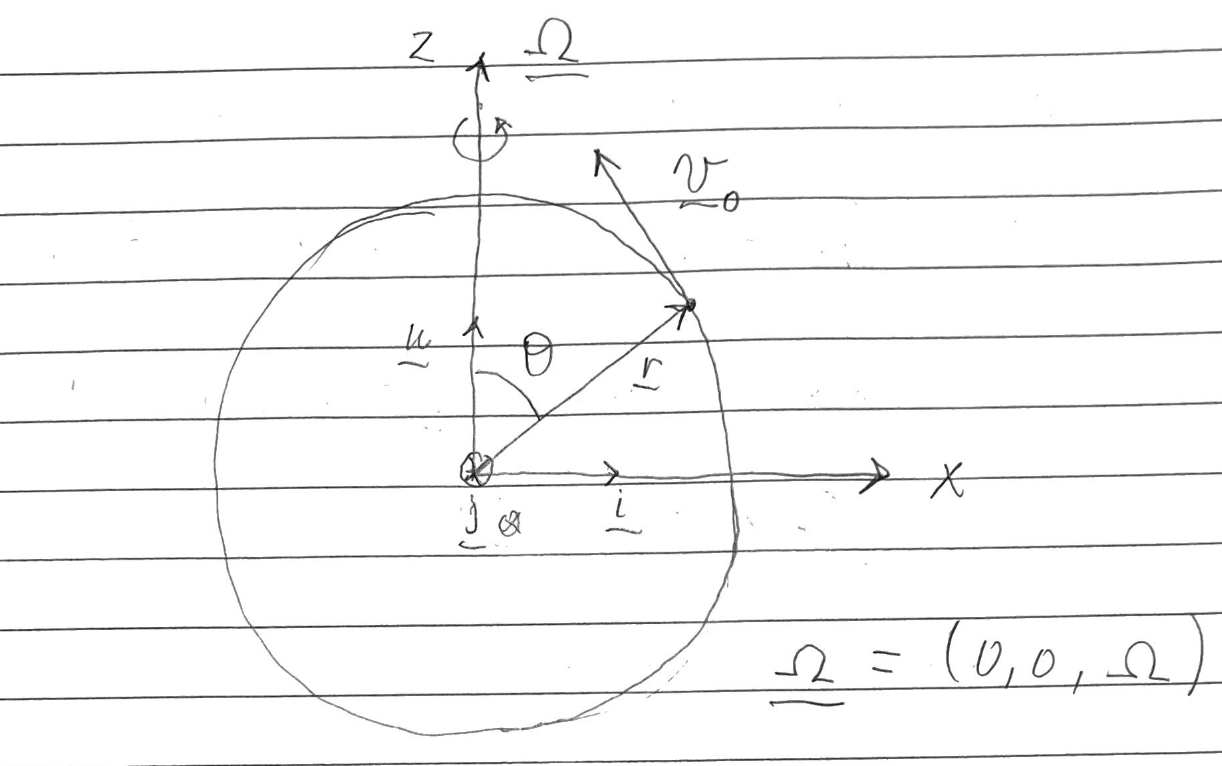
\includegraphics[width=0.8\linewidth]{../figures/F17_9_9.png}
  \label{fig:F17_9_9}
\end{figure}

Vi har generelt at Coriolis-kraften er givet som
\[ 
F_{cor} = 2m \Vec{v_0} \times \Vec{\Omega}
.\]
Og krydsproduktet $\Vec{v_0} \times \Vec{\Omega}$ er givet ved
\[ 
\Vec{v_0} \times \Vec{\omega} = v_0 \cdot \cos(\theta) \cdot \Omega
.\]
Vi har dermed at
\[ 
F_{cor} = 2m \cdot v_0 \cdot \cos(\theta) \cdot \Omega
.\]

Fra højrehåndsreglen må det i øvrigt gælde at Corioliskraftens retning er mod højre (se evt. \textbf{\autoref{fig:F17_9_9}}). For at finde $\frac{a_{cor}}{g}$ regner vi først jordens omdrejningshastighed som
\[ 
\Omega = \frac{2 \pi}{\qty{24}{hr} \cdot \qty{3600}{\frac{s}{hr}}} = \qty{7,2722e-5}{s^{-1}} 
.\]
Vi kan dermed regne $\frac{a_{cor}}{g}$ som
\[ 
\frac{a_{cor}}{g} = 2v_0 \cdot \cos(\theta) \cdot \Omega = 2\cdot \qty{1000}{\frac{m}{s}} \cdot \cos(\ang{40}) \cdot \qty{7,2722e-5}{s^{-1}} \cdot \frac{1}{\qty{9,81}{\frac{m}{s^2}}} = \num{0,0114} 
.\]
Altså er størrelsen på Corioliskraften lidt over 1\% så stor som kuglens tyngdekraft.


\section*{Opg. 9.10}
The derivation of the equation of motion for a rotating frame made the assumption that the angular velocity $\Omega$ was constant. Show that if $\dot{\Omega} \neq 0$ then there is a third ``fictuous force,'' sometimes called the \textit{azimuthal force}, on the right side of (9.34) equal to $mr \times \dot{\Omega}$
\bigbreak
Fra Taylor-notatet haves at
\begin{align*}
  \left( \frac{\mathrm{d}r}{\mathrm{d}t}  \right)_{S_0} &= \left( \frac{\mathrm{d}r}{\mathrm{d}t}  \right)_S + \sum r_i \left( \frac{\mathrm{d} \Vec{e}_i}{\mathrm{d}t}  \right)_{S_0} \\
  &= \dot{r} + \sum r_i(\Vec{\Omega} \times \Vec{e}_i)  \\
  &= \dot{r} + \Vec{\Omega} \times r \\
  &= \dot{r} + \Vec{\Omega} \times \Vec{r}
\end{align*}
Der differentieres igen så vi får at
\[
\left( \frac{\mathrm{d}^2 \Vec{r}}{\mathrm{d}t^2}  \right)_{S_0} = \ddot{\Vec{r}} + \dot{\Vec{\Omega}} \times \Vec{r} + \Vec{\Omega} \times \dot{\Vec{r}} + \Vec{\Omega} \times \dot{\Vec{r}} + \Vec{\Omega} \times (\Vec{\Omega} \times \Vec{r})
.\]
Hvilket kan skrives som
\[ 
  \ddot{r} = \Vec{r} \times \Vec{\Omega} + 2\dot{\Vec{r}} \times \Vec{\Omega} + \left( {\Vec{\Omega}} \times \Vec{r} \right) \times \Vec{\Omega}
.\]
Og dermed fås at $N2$ er
\[ 
  N2 = m \ddot{r} = \Vec{F} + m \Vec{r} \times \dot{\Vec{\Omega}} + 2m \dot{\Vec{r}} \times \Vec{\Omega} + m \left( \Vec{\Omega} \times \Vec{r} \right) \times \Vec{\Omega}
.\]

\section*{Opg. 9.12}

\subsection*{(a)}
Show that to design a static structure in a rotating frame (such as a space station) one can use the ordinary rules of statics except one must include the extra ``fictitous'' centrifugal force. 
\bigbreak
Vi opskriver Newtons 2. lov for et roterende system
\[ 
m \ddot{\Vec{r}} = \Vec{F} + 2m \dot{\Vec{r}} \times \Vec{\Omega} + m(\Vec{\Omega} \times \Vec{r}) \times \Vec{\Omega}
.\]
I det statiske tilfælde har vi at
\[ 
\Vec{0} = \Vec{F} + m (\Vec{\Omega} \times \Vec{r}) \times \Vec{\Omega}
.\]
Altså ses at centrifugalkraften overlever, selv for det statiske tilfælde.


\subsection*{(b)}
I wish to place a puck on a rotating horizontal turntable (angular velocity $\Omega$) and to have it remain at rest on the table, held by the force of static friction (coefficient $\mu$). What is the maximum distance from the axis of rotation at which I can do this? (Argue from the point of view of a observer in the rotating frame.)
\bigbreak
For statik har vi at $\sum F_r = 0$. Altså har vi at
\begin{align*}
  mr \Omega^2 - mg\mu &= 0 \\
  g\mu &\geq r\Omega^2 \\
  r &\leq \frac{g\mu}{\Omega^2}
.\end{align*}


\section*{Opg. 6-3}
En partikel kan bevæge sig uden gnidning på en vandret flade. På grund af Jordens rotation, vil partiklen fjerne sig fra startsituationens tangent. Stedets bredde er \ang{60}. Partiklens hastighed er \qty{16,0}{m/s}. Det antages, at corioliskraftens størrelse og retning er konstant under bevægelsen. Beregn hvor langt partiklen i løbet af \qty{10}{s} vil fjerne sig startsituationens tangent.
\bigbreak
Coriolisaccelerationen er givet som
\[ 
a_{cor} = 2v \Omega \sin(\beta)
.\]
Hvor $\beta$ er breddegraden. Vi har generelt jordens omdrejningshastighed som
\[ 
\Omega = \frac{2\pi}{24 \cdot 3600} = \qty{7,272e-5}{\frac{rad}{s}}
.\]
Vi har desuden, at $\sin(\ang{60}) \approx \num{0,866}$ og $v = \qty{16,0}{\frac{m}{s}}$. Dermed fås
\[ 
a_{cor} = 2v \Omega \sin(\beta) = \qty{2,015e-3}{\frac{m}{s^2}} 
.\]
Denne acceleration er konstant og derfor kan formlen for konstant acceleration bruges til at finde den samlede bevægelse i løbet af $\Delta t = \qty{10}{s}$ som
\[ 
\Delta x = \frac{1}{2}a_{cor}(\Delta t)^2 = \qty{0,101}{m}
.\]

\section*{Opg. 6-4}
En lastbil starter fra hvile til tiden $t = 0$ og accelererer jævnt, således at dens fart er $v_1 = \qty{20}{\frac{m}{s}}$ til tiden $t = t_1 = \qty{10}{s}$. En lille kasse med massen $m = \qty{5,0}{kg}$ er før starten anbragt i afstanden $\ell = \qty{3,0}{m}$ fra bagenden. Til $t = 0$ begynder kassen at glide. Gnidningskoefficienten mellem kasse og lad er $\mu_k = 0,15$.

\subsection*{(a)}
Angiv de kræfter, der virker på kassen såvel i bilens som i vejbanens henførelsessystem.
\bigbreak
I begge tilfælde virker følgende kræfter
\begin{itemize}
  \item Tyngdekraft: $mg$ 
  \item Normalkraft: $N$
  \item Gnidningskraft: $F_{\mu}$
\end{itemize}

\subsection*{(b)}
Find kassens acceleration i begge henførelsessystemer
\bigbreak
Normalkraften, $N$, er givet som
\[ 
N = mg
.\]
Vi har dermed også et udtryk for gnindningskraften, $F_{\mu}$, som
\[ 
F_{\mu} = ma = mg\mu \implies a = g\mu = \qty{1,47}{\frac{m}{s^2}} 
.\]

For at finde accelerationen i det accelererende koordinatsystem benyttes Newtons 2. lov for et accelererende koordinatsystem
\begin{align*}
  ma' &= F_{\mu} + (-ma_0) = 0 \\
  a' &= g\mu - a_0 \\
     &= \qty{9,81}{\frac{m}{s^2}} \cdot \num{0,15} - \frac{\qty{20}{\frac{m}{s}}}{\qty{10}{s}}  \\
     &= \qty{-0,53}{\frac{m}{s^2}}
.\end{align*}


\subsection*{(c)}
Bestem den tid, som kassen er om at nå bagenden.
\bigbreak
Vi har den generelle formel for bevægelse ved konstant acceleration som
\begin{align*}
  \ell &= \frac{1}{2} |a'|t^2 \\
  \implies t &= \sqrt{\frac{2 \ell}{|a'|}} \\
  &= \sqrt{\frac{2\cdot \qty{3,0}{m}}{\qty{0,53}{\frac{m}{s^2}}}} \\
  &= \qty{3,36}{s}
.\end{align*}


\subsection*{(d)}
Find den vandrette komposant af kassenss hastighed, når kassen rammer vejen.
\bigbreak
Kassen kan kun blive accelereret når den ligger på bilens lad og der antages ingen luftmodstand og derfor vil bilens hastighed være konstant fra den forlader bilen til den rammer vejen. Altså kan den vandrette hastighed findes med den almindelige formel for hastighed ved konstant acceleration som
\begin{align*}
  v &= at \\
  &= \qty{1,47}{\frac{m}{s^2}} \cdot \qty{3,36}{s}  \\
  &= \qty{4,94}{\frac{m}{s}} 
.\end{align*}


\section*{Opg. 6-9}
En dødsdrom er en lodretstående cylinder, på hvis indre overflade en motorcyklist kan køre rundt. Tidligere har dødsdromer været populære forlystelser på omrejsende markeder. I en dødsdrom med radius $ R = \qty{4}{m}$ kører en motorcyklist med hastigheden $v = \qty{40}{\frac{km}{h}}$

\subsection*{(a)}
Vis, at denne bevægelse er mulig?
\bigbreak
\begin{figure}[ht]
  \centering
  \incfig[0.8]{F17_3}
  \caption{Skitse over situationen, der viser at bevægelsen er mulig.}
  \label{fig:F17_3}
\end{figure}
Se \textbf{\autoref{fig:F17_3}}

\subsection*{(b)}
Hvilken hældning har cyklen med lodret?
\bigbreak
Først findes cyklens centripetalacceleration, for at kunne bruge trigonometri til at finde vinklen til lodret $\theta$. Dette gøres som
\begin{align*}
  a_{cp} &= \frac{v^2}{R} \\
  &= \frac{\left( \qty{40}{\frac{km}{h}}  \right)^2}{\qty{4}{m}} \\
  &= \qty{30,86}{\frac{m}{s^2}} 
.\end{align*}
Vha. trigonometri kan vinklen til lodret da findes som
\begin{align*}
  \theta &= \tan^{-1} \left( \frac{-a_{cp}}{-g} \right) \\
  &= \tan^{-1} \frac{\qty{30}{\frac{m}{s^2}}}{\qty{9,80}{\frac{m}{s^2}}} \\
  &= \num{0,307} \cong \ang{17,62} 
.\end{align*}


\subsection*{(c)}
Hvilket effektivt tyngdefelt føler cyklisten?
\bigbreak
Det effektive tyngdefelt er blot den effektive acceleration. Altså har vi
\[ 
g_{eff} = \sqrt{a^2 + g^2} = \sqrt{\left( \qty{30,86}{\frac{m}{s^2}}  \right)^2 + \left( \qty{9,80}{\frac{m}{s^2}} \right)^2} = \qty{32,38}{\frac{m}{s^2}}  
.\]


\subsection*{(d)}
Beskriv, hvordan det må føles at køre i dødsdrom. (G)
\bigbreak
Vi finder forholdet mellem det effektive tyngdefelt og det normale tyngdefelt som
\[ 
G = \frac{g_{eff}}{g} = \frac{\qty{32,38}{\frac{m}{s^2}}}{\qty{9,80}{\frac{m}{s^2}}} = \num{3,3}G
.\]


\end{document}
